
\chapter{From Action to Reaction: Latent Space Regularization and Alignment for Human Reaction Motion Generation with Intermediate Motion Semantics}

\section{Summary}
Creating lifelike virtual humanoids capable of simulating reactive movements towards humans or other characters holds ...

\section{Introduction}
Human motion generation is at the core of many applications in computer animation, augmented/virtual reality, robotics,...


\begin{figure*}[t]	
	\centering
	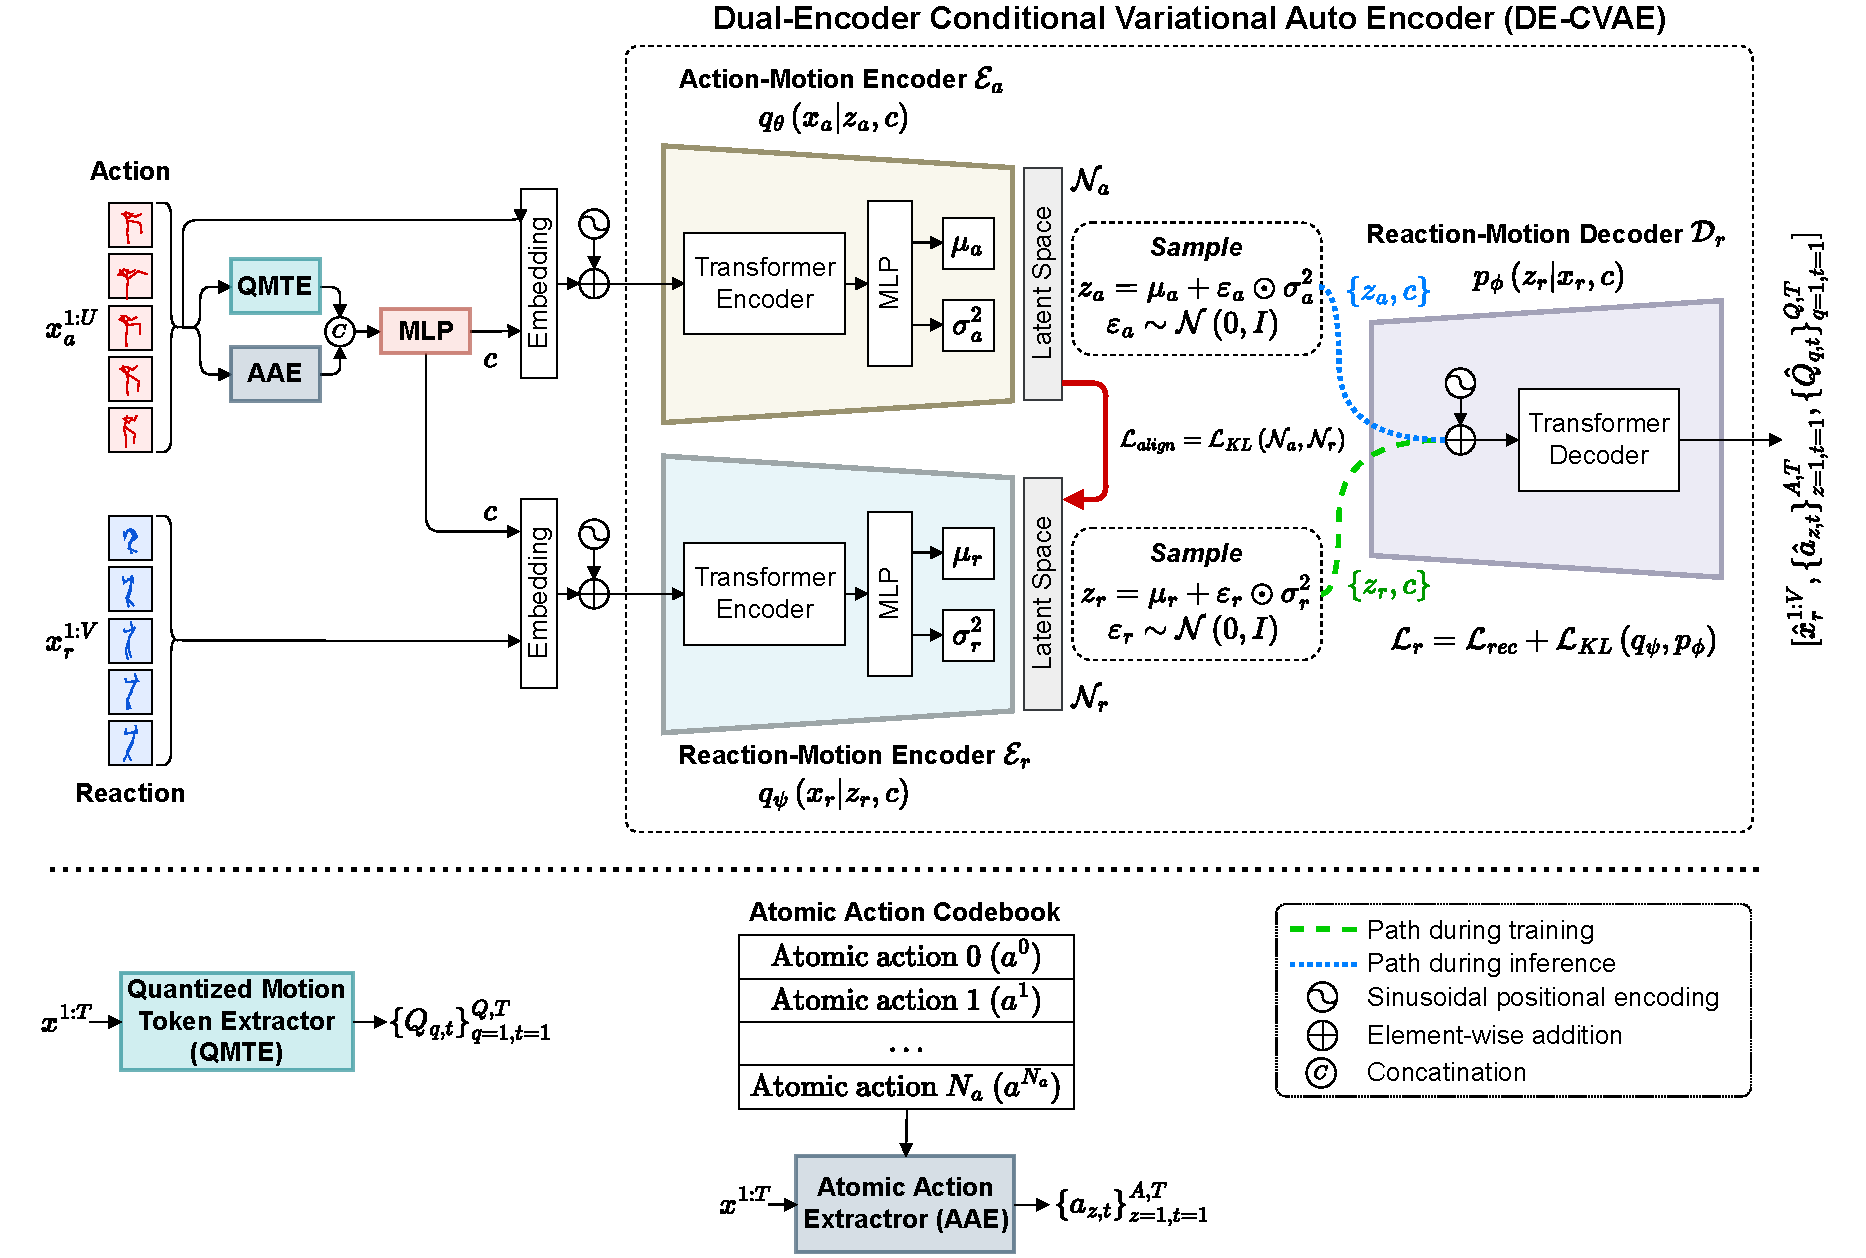
\includegraphics[width=1\textwidth]{figures/chapter4/fig_overview}
	\caption{Overview of the proposed model (left) DE-CVAE network with two encoders and a decoder. QMTs and atomic action vectors are extracted from action-motion using QMTE and AAE modules, respectively (right) QMTE module, AAE module, and atomic action codebook.}
	\label{fig_overview}
\end{figure*}


\section{Related Work}
\subsection{Human Motion Generation}
The human motion generation task aims to produce realistic motion sequences for individuals or interactions involving humans...


\begin{sidewaysfigure}	
	\centering
	\includegraphics[width=0.8\textwidth]{figures/chapter4/fig_qmt}
	\caption{(Top left) Motion sequence (top middle) orientational and positional quantizations (top right) extracted quantized motion tokens (bottom) visual representations for QPT, QPRPT, QPDT, QLAT, QLOT, and QJVT.}
	\label{fig_qmt}
\end{sidewaysfigure}

\section{Method}
\subsection{Problem Formulation}
The human reaction-motion generation task aims to accurately generate the 3D skeleton-based motion of a character, given the action-motion sequence of another character. In the training phase, the input comprises action and reaction motion pairs $ \left\lbrace \left( x_a^{1:U},x_r^{1:V}\right) \right\rbrace  $, where $ x_a^{1:U} $ and $ x_r^{1:V} $ are the action and corresponding reaction-motion sequences, respectively. The motion sequence $ x^{1:T}=\left[ S_1,\dots ,S_T\right]  $ is represented as the human skeleton sequence defined for each discrete time interval $t \in \left\lbrace 1,\dots,T\right\rbrace  $, where $ S_t \in \mathbb{R}^{J \times 3} $ is the human skeleton configuration at any given time $ t $ with $ J=15 $ 3D joint keypoints. Conversely, during the inference phase, our learned model can be expressed as a motion-motion translation function $ G: x_a^{1:U} \rightarrow x_r^{1:V} $.

\subsection{Overview}
The overall pipeline of the proposed method is shown in Fig. \ref{fig_overview}. The method uses an action-motion sequence $ x_a^{1:U}$ and extracts quantized motion tokens and atomic action vectors to generate the conditional signal. The two encoders and a decoder use this conditional signal as a bias to disentangle and regularize the motion spaces. This results in a improved the action-reaction mapping. The reaction-motion encoder encodes ...


\begin{equation}
	\label{eq1}
	{QPT}_t^{(j,\dagger)} = \left\langle {\frac{ s_t^j - s_t^0}{{q_l^p}} }, \frac{{r_t^\dagger}}{{q_l^p}} \right\rangle  - \left\langle \frac{{s_{t-1}^j - s_{t-1}^0}}{{q_l^p}}, \frac{{r_{t-1}^\dagger}}{{q_l^p}} \right\rangle
\end{equation}





\section{Implementation Details}
\label{implementation}
The model was implemented using the open-source PyTorch library. Network weights were initialized randomly and optimized using the Adam optimizer employing a mini-batch size of 32 for 45K epochs. The initial learning rate was set to $ \alpha=10^{-5} $ and decayed gradually with the Step LR scheduler with a step size of 8 and decay rate ...


\section{Experiments}
\label{exp_res}

\subsection{Datasets}
\label{datasets}

\noindent
\textbf{SBU Kinect Interaction Dataset (SBU) \cite{sbu_dataset}} features a skeleton-based two-person interaction dataset collected from the actions of seven individuals organized in 21 pairs of two-actor sets...

\noindent
\textbf{Kinect-based 3D Human Interaction Dataset (K3HI)\cite{k3hi_dataset}} offers a comprehensive repository of rich ...



\begin{sidewaysfigure}	
	\centering
	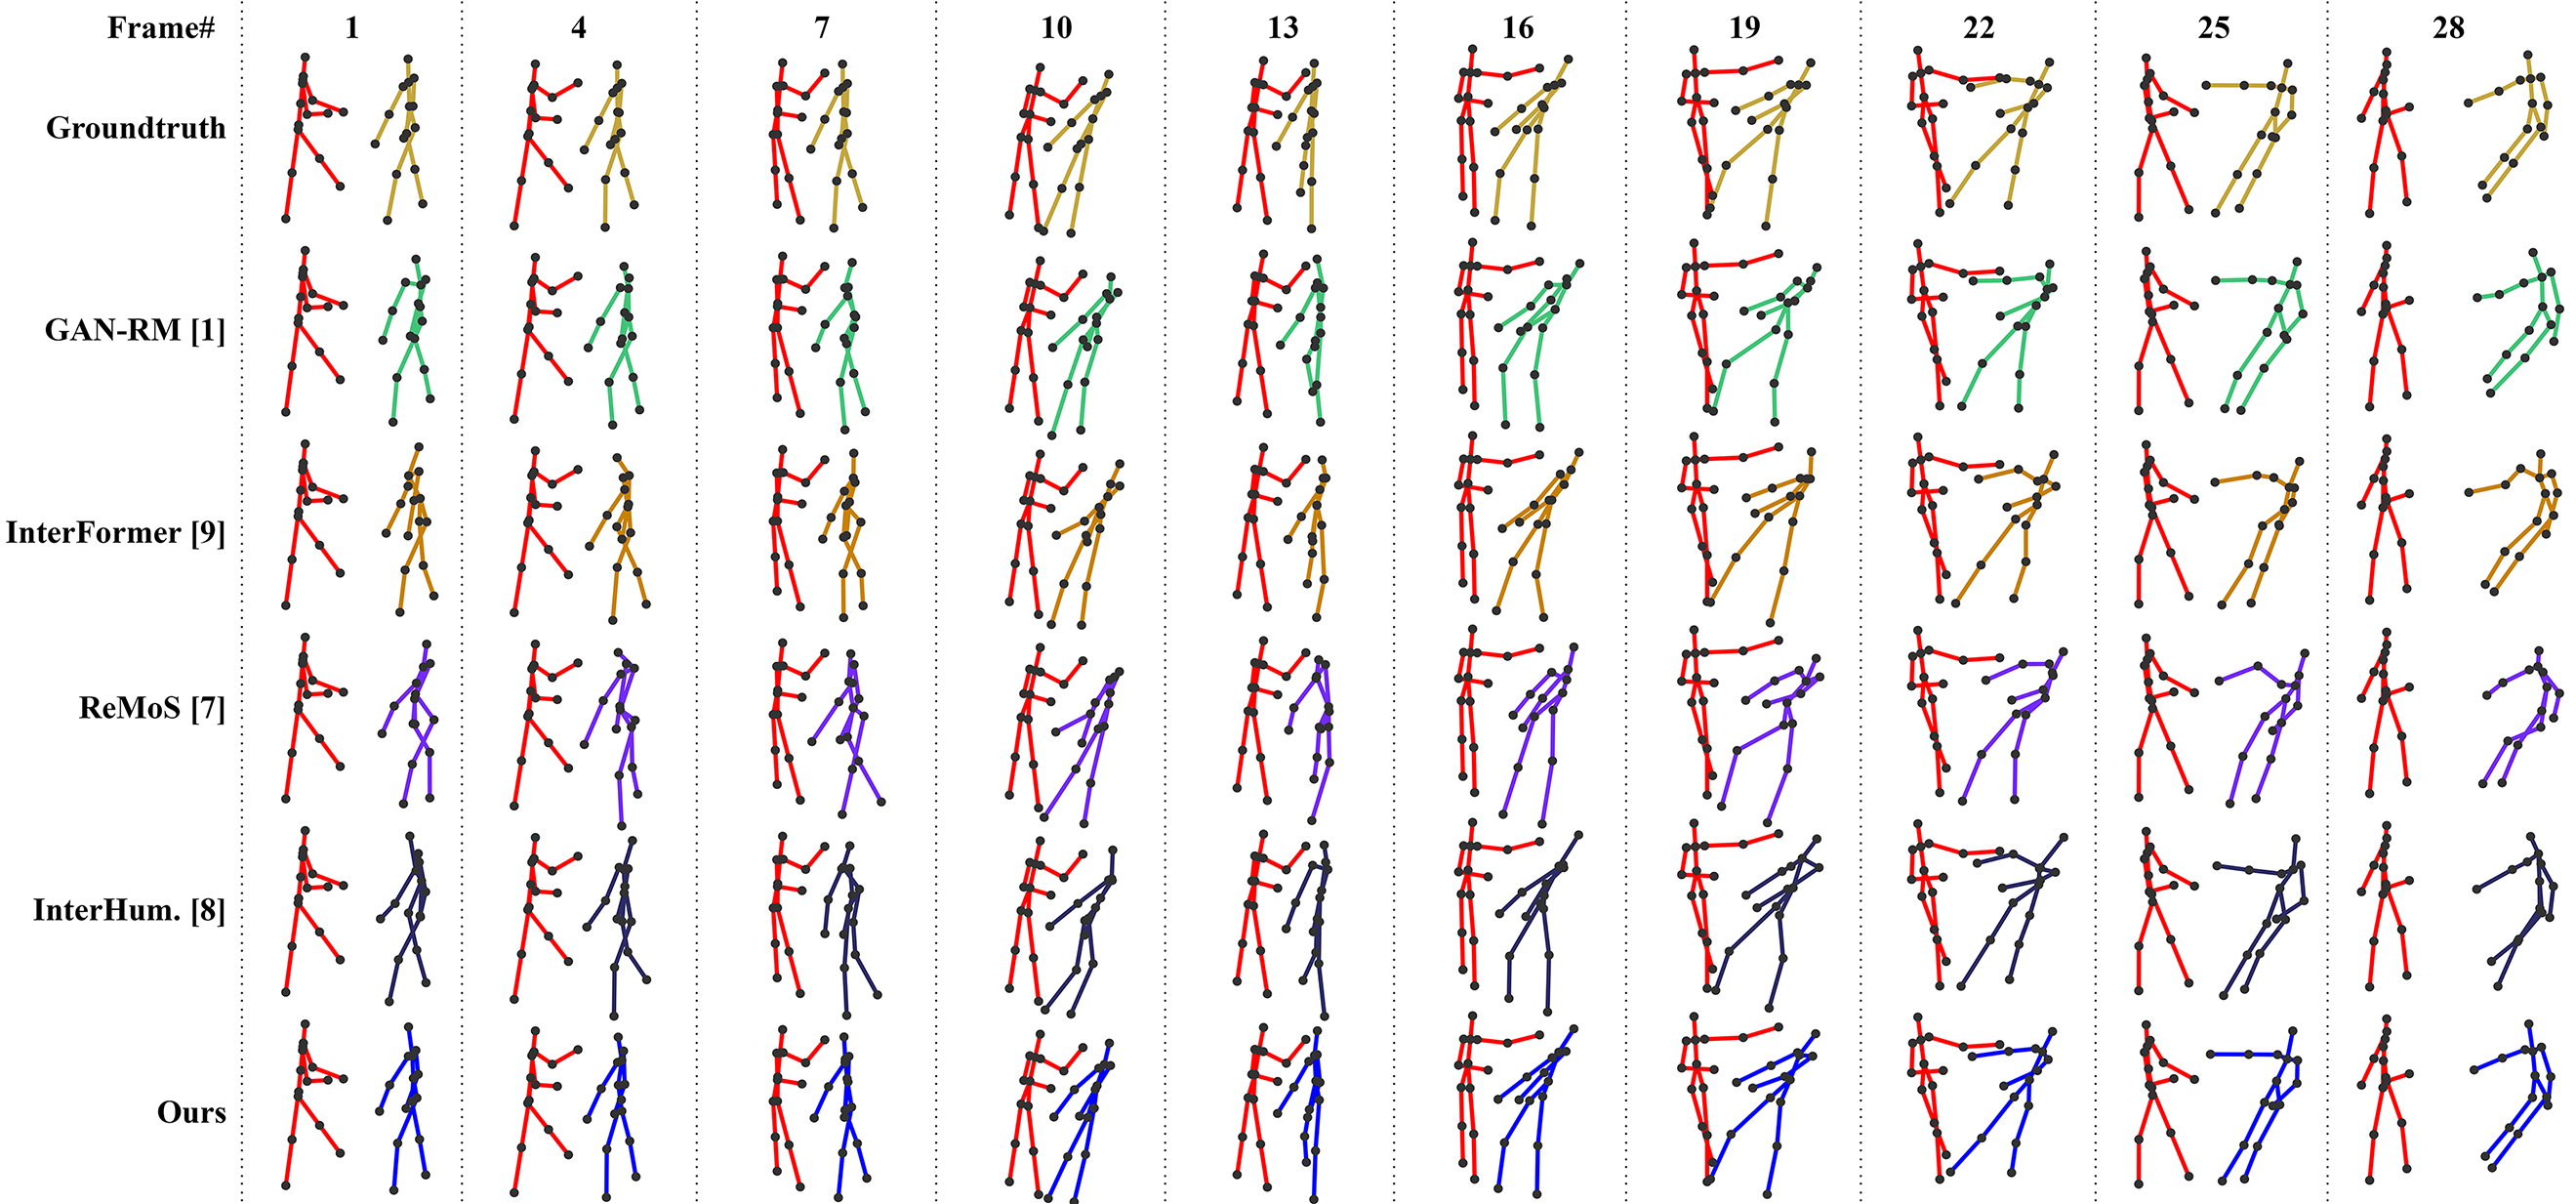
\includegraphics[width=0.9\textwidth]{figures/chapter4/fig_results_sbu}
	\caption{Visualization of motion generation on SBU dataset for punching class. Skeletons in red represent acting character, while the other colors correspond to the reacting character in various methods. (top to bottom) represent motion sequences for groundtruth, generated by methods \cite{gan-reaction-motion}, \cite{interaction_transformer}, \cite{remos}, \cite{interaction-humanoid}, and our results, respectively. (left to right) selective frames during temporal transition.}
	\label{fig_results_sbu}
\end{sidewaysfigure}



\subsection{Evaluation Metrics}
\label{evaluation}

Due to the inherent nature of reaction-motion generation, it is a one-to-many mapping problem...

\noindent
\textbf{The Fr'echet Motion Distance (FMD)} is specifically designed to measure the distance between ground truth and generated data distribution...



\subsection{State-of-the-Art Comparisons}
\label{sota}

\noindent
\textbf{Quantitative Evaluation.} We conducted a comprehensive evaluation of the proposed method by comparing the FMD and diversity evaluation scores on the SBU, DuetDance, and K3HI datasets, as summarized in Table. \ref{table_sota_fmd_div}...






\begin{sidewaystable}
	\centering
	\caption{(Left) Classification accuracy for each class in the SBU, Duetance, and K3HI datasets, comparing our method with groundtruth and exiting approaches (\cite{gan-reaction-motion}, \cite{remos}, \cite{interaction-humanoid}, \cite{interaction_transformer}, \cite{intergen}, and \cite{social-robot}) (right) user perception study, comparing our methods with groundtruth and existing approaches (\cite{interaction_transformer} and \cite{gan-reaction-motion}) across the same datasets. $"\uparrow"$: indicates higher is better. \textbf{Bold} specifies the best results.}
	\label{table_sota_classification_user}
	\renewcommand{\arraystretch}{1.0}
		\begin{tabular*}{1.0\textwidth}{@{\extracolsep{\fill}}l|cccccccc|cccc}	
			\toprule			
			\multirow{2}{*}{Method} &
			GT  &
			GAN-RM  &
			ReMoS  &
			InterHum.  &
			InterFor.  &
			InterGen  &
			Social Rob. &
			Ours &
			GT &
			InterFor. &
			GAN-RM &
			Ours \\ 
			
			&
			&
			\cite{gan-reaction-motion} &
			\cite{remos} &
			\cite{interaction-humanoid} &
			\cite{interaction_transformer} &
			\cite{intergen} &
			\cite{social-robot} &
			&
			&
			\cite{interaction_transformer} &
			\cite{gan-reaction-motion} &
			\\ \hline
			
			\multicolumn{9}{c}{Classification Accuracy $(\uparrow)$} &
			\multicolumn{4}{c}{User Preference $(\uparrow)$} \\ 
			\midrule
			
			\multicolumn{13}{c}{SBU Kinect Interact} \\ 
			\midrule
			
			
			
			
			Walking &89&75&63&60&76&53&44&\textbf{85}&95\%&77\%&80\%&\textbf{89\%}\\
			Kicking &100&\textbf{94}&79&68&82&75&77&93&92\%&\textbf{85\%}&78\%&81\%\\
			Pushing &94&75&71&70&83&68&71&\textbf{91}&88\%&77\%&\textbf{78\%}&73\%\\
			Shaking Hands &97&\textbf{91}&72&67&82&73&71&87&86\%&70\%&73\%&\textbf{82\%}\\
			Exchanging &95&\textbf{89}&69&82&72&66&67&88&89\%&78\%&\textbf{88\%}&76\%\\
			Punching &100&90&78&75&88&78&76&\textbf{93}&93\%&72\%&75\%&\textbf{90\%}\\
			Average &95.83&85.67&72&70.33&80.5&68.83&67.67&\textbf{89.5}&90.5\%&76.5\%&78.67\%&\textbf{81.83\%}\\ 
			\midrule
			
			\multicolumn{13}{c}{DuetDance} \\ 
			\midrule
			
			
			
			
			Cha-Cha &94&80&73&68&74&69&53&\textbf{87}&88\%&74\%&76\%&\textbf{82\%}\\
			Jive &95&86&70&71&81&69&73&\textbf{93}&79\%&62\%&\textbf{76\%}&74\%\\
			Rumba &92&78&66&67&78&67&64&\textbf{85}&78\%&68\%&66\%&\textbf{74\%}\\
			Salsa &97&\textbf{93}&75&73&78&70&71&92&84\%&66\%&75\%&\textbf{79\%}\\
			Samba &96&77&74&69&\textbf{89}&71&60&82&85\%&75\%&70\%&\textbf{83\%}\\
			Average &94.8&82.8&71.6&69.6&80&69.2&64.2&\textbf{87.8}&82.8\%&69\%&72.6\%&\textbf{78.4\%}\\ 
			\midrule
			
			\multicolumn{13}{c}{K3HI} \\ 
			\midrule
			
			
			Approaching &98&84&72&78&78&72&65&\textbf{97}&88\%&74\%&78\%&\textbf{81\%}\\
			Departing &93&90&68&82&66&69&68&\textbf{93}&84\%&72\%&76\%&\textbf{80\%}\\
			Kicking &100&82&72&93&76&75&70&\textbf{94}&89\%&\textbf{86\%}&76\%&85\%\\
			Pushing &100&\textbf{96}&77&84&76&72&74&95&89\%&78\%&74\%&\textbf{85\%}\\
			Shaking &96&\textbf{94}&68&75&75&71&71&90&87\%&76\%&78\%&\textbf{84\%}\\
			Exchanging &93&77&72&84&70&69&48&\textbf{93}&90\%&78\%&\textbf{88\%}&86\%\\
			Punching &100&89&75&90&82&71&74&\textbf{94}&90\%&72\%&80\%&\textbf{89\%}\\
			Pointing &94&81&68&87&66&70&67&\textbf{89}&86\%&73\%&\textbf{86\%}&84\%\\
			Average &96.75&86.62&71.5&84.12&73.62&71.125&67.12&\textbf{93.12}&87.87\%&76.12\%&79.5\%&\textbf{84.25\%}\\ 
			\midrule
			
	\end{tabular*}
\end{sidewaystable}


\noindent
\textbf{Qualitative Evaluation.} We performed a qualitative evaluation by visually comparing the motion sequences generated by the proposed method with the groundtruth and various SOTA methods. Fig. \ref{fig_results_sbu}, \ref{fig_results_k3hi}, and \ref{fig_results_duetdance} show the qualitative comparisons of the test samples from ...


\noindent
\textbf{Perceptual User Study.} Relying solely on quantitative evaluation and self-performed qualitative analysis is insufficient due to the intricacies of the problem at hand. For a more comprehensive visual assessment of motion quality, ...


\subsection{Ablation Study}
\label{ablation}
To assess the effectiveness of the proposed modules in our network, we performed an ablation study on the SBU dataset, focusing on the diversity and FMD metrics. We set up four versions of our model and tested them with different ... 

\section{Conclusion}
\label{conclusion}
In this paper, we introduce a novel DE-CVAE network featuring two encoders designed for the task of human reaction motion generation... 


\section{Future Work}
\label{future}
Despite significant improvements in the generation task, our approach faces three major challenges. (1) As the interactions...


